%%%%%%%%%%%%%%%%%%%%%%%%%%%%%%%%%%%%%%%%%%%%%%%
\chapter{Decoding FEC Chain} \label{chap:DecodingChain}
%%%%%%%%%%%%%%%%%%%%%%%%%%%%%%%%%%%%%%%%%%%%%%%
In this chapter, implementation and optimization details of 5G polar decoding FEC are presented including challenges faced while achieving low latency decoding. In FEC chain, decoder is the critical part due to inherent sequential nature of polar decoding. $n^{th}$ bit is decoded by using all the previously decoded bits, hence $n^{th}$ bit depends on $0$ to $n-1$ bits. Due to sequential decoding process, significant latency is introduced by the decoder. This section presents the optimization techniques employed to improve decoding FEC chain latency, which include both algorithmic and platform specific optimizations. Each these techniques are explained in the respective sections where these are employed. In this work, FEC chain considered is part of the base station, therefore uplink control information is decoded at receiver. PUCCH (Physical uplink control channel) and PUSCH (Physical uplink shared channel) contain polar encoded information. Received signal after demodulation is quantized to 16-bit LLR (log likelihood ratio) values. Decoding is performed with LLR (Log likelihood ratio) values rather than probabilistic likelihoods due to their numerical stability and low computational complexity. Receiver side FEC chain is a reverse of the operations performed at transmitter. Figure ~\ref{fig:5grx_fec_chain} shows the receiver side polar decoding FEC chain.

\begin{figure}[]
	\centering
	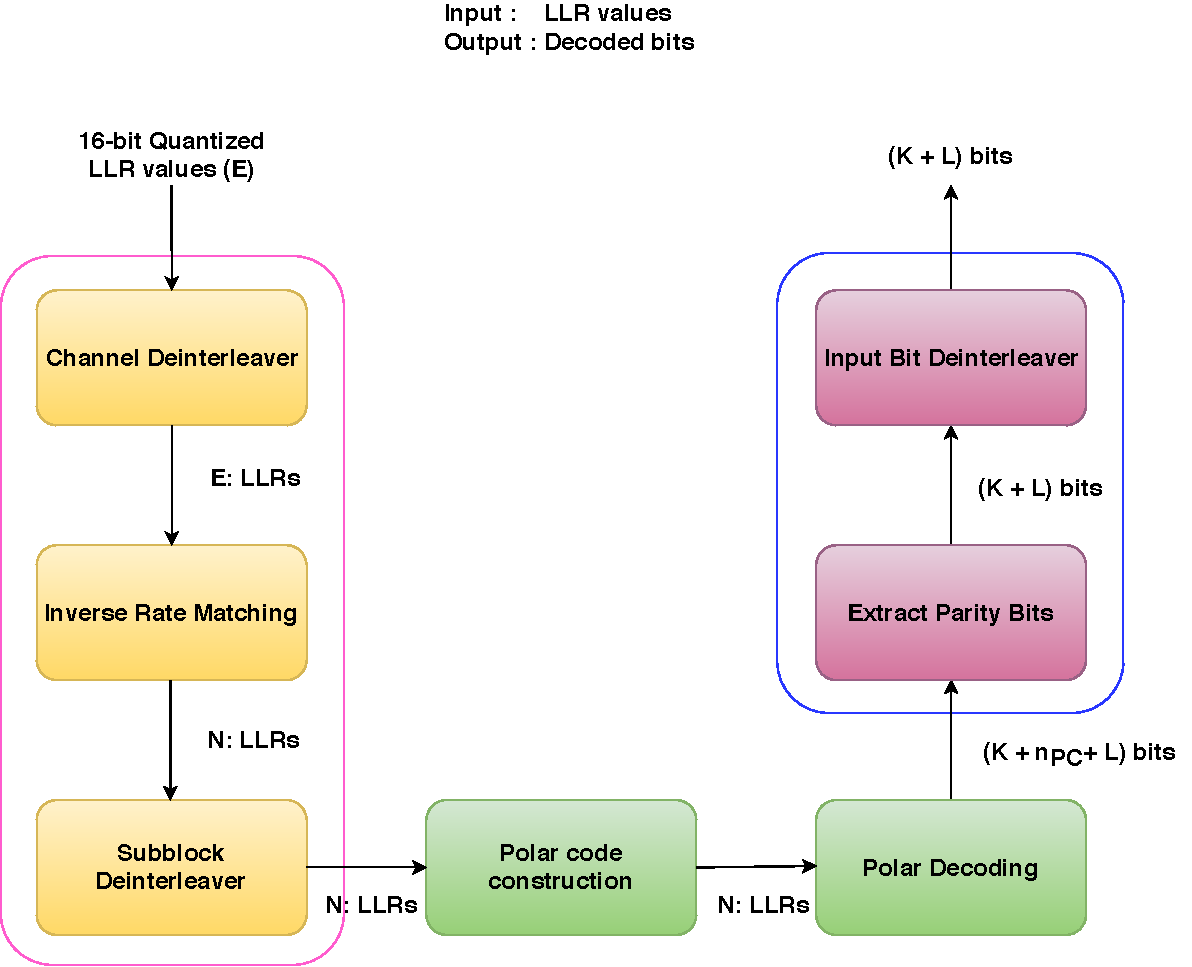
\includegraphics[width=0.7\textwidth]{./figures/receiverFECChain.pdf}
	\caption{Polar decoding FEC chain for PUCCH/PUSCH}
	\label{fig:5grx_fec_chain}
\end{figure}

%$\mathtt{Yadhu}$
%\NOTE{Decoding is of serial nature, has lot of latency. Polar decoding chain necessity. PUCCH and PUSCH, parameters of both the channels.}
%%	Explain all the decoding Optimizations I have done, In this document.
%% 	Explain of the latency without optimization.

\section{Decoding algorithms}
The basic decoding algorithm successive cancellation (SC) is developed by the Arikan in his seminal work on polar codes \cite{Arikan}. It achieves the symmetrical capacity of binary memoryless channel through sequential decoding when block length is very large. However due to the sequential nature significant latency is introduced by decoding algorithm. Latest 5G standard specifies transmission time interval (TTI) of $125 \mu s$ \TODO{cite the doc}, within this duration scheduling and encoding/decoding must be done. Therefore it is very important to efficiently perform FEC chain operations. This work concentrates on implementing the polar encoding/decoding in software and studies the feasibility of satisfying the strict latency requirements of 5G. Decoding through SC algorithm can be represented as binary tree, decoding process is nothing but traversing through a tree sequentially. Significant research work is done both in academia and industry to improve decoding latency of the SC algorithm. Major improvement to SC which significantly reduced the decoding latency is identifying special kind nodes in a tree which allow immediate decoding of multiple bits without requiring full tree traversal. Algorithms presented in \cite{SSC} and \cite{fastSSC} present such improvements, which identify special nodes or in other words component codes such as \textit{Rate-0}, \textit{Rate-1}, \textit{RPC} and \textit{SPC} nodes, \textit{RPC} and \textit{SPC} mean repetition and single parity check code respectively. Identification of special nodes requires finding particular patterns the frozen bit locations in the constructed polar code. To gain full advantages of Fast-SSC (Fast Simplified Successive Cancellation) algorithm, special nodes must be identified efficiently. In this work, 5G RX FEC chain with fast-SSC algorithm implemented/optimized in software and feasibility of achieving desired latency( $< 50\mu s$) is analyzed.
%Following sections present how processor specific features are exploited to efficiently identify


\section{Decoding chain}
The figure ~\ref{fig:5grx_fec_chain} shows the complete receiver side FEC chain. It is almost a inverse operations of encoding FEC chain except few differences related to PUCCH and PDSCH which contain parity check bits ($ n_{PC} $). The decoding FEC chain receives UCI(Uplink Control Information) in the form of 16-bit quantized $ E $ LLR values. Before passing LLR values to decoder inverse operations of the steps which were carried out aftermath of encoding, which are channel deinterleaving, inverse rate matching and subblock deinterleaving. These steps grouped by a pink rectangle in the figure, after these steps polar code construction is performed using same optimized method as presented in the previous chapter. Polar code construction procedure outputs the information bit positions, from which frozen pattern can be obtained. Next step in the FEC chain is polar decoding, $ N $ LLR values and frozen pattern is passed to polar decoder, which outputs the decoded bits. Polar construction and decoding blocks are colored green the FEC chain figure. Using information bit positions obtained in the polar construction procedure $ K + n_{PC} + L $ bits are extracted from $ N $ decoded bits. $ K + n_{PC} + L $ bits contain $ n_{PC} $ parity bits, extracting these bits requires identifying the row of minimum weight from the generator matrix of polar code. Finally input deinterleaving is applied on the remaining $ K +  L $ bits to obtain concatenated information and CRC bits. Blocks representing Extracting parity bits and input bit deinterleaver are grouped with blue rectangle. In this section, we presented briefly the functionalities carried out by different blocks of the decoding FEC chain. Next we will analyze the latency contributions of each those operations and come up with optimizations both algorithmic and platform specific to reduce latency.

\section{Channel deinterlever}
The first operation after receiving the LLR values is channel deinterleaving, This is the exact inverse of the interleaving operation done at the transmitter. Channel interleaving is performed to make transmission robust against burst errors. Authors of \cite{3gpp.TSG-RAN_WG1} analyze the error correction performance of polar codes for different channel conditions and constellations. It is found that error correction performance significantly deteriorates for constellations 16-QAM onwards. Channel interleaving wasn't done for downlink PBCH/PDCCH since the constellation was QPSK, however in case of PUCCH/PUSCH higher constellations are used hence channel interleaving is necessary. In 5G standard  isosceles right triangle interleaver is adopted. Deinterleaving is carried out by writing LLR values to columns of triangular structure and reading LLR values in rows. Interleaver design is proposed by Qualcomm \cite{3gpp.TSG-RAN_WG1}.

Vector processing instructions cannot be used for the implementation of interleaver due irregular and non uniform memory access, therefore interleaver just plain functional implementation. One optimization technique was to avoid new memory allocation and using already allocated memory. This avoids the overhead of dynamic memory allocation and initialization. Channel deinterleaving is one of significant contributor to latency in polar decoding FEC chain, since each of the LLR values need to processed sequentially.

\section{Inverse rate matching}
Inverse rate matching step maps the $E$ LLR values to mother code block size $ N $. Rate matching step has three modes puncturing, shortening and repetition. Mode is selected based on rate matcher output size ($E$) and mother code size($ N $). If $E > N$ then repetition performed, otherwise either puncturing and shortening is done. If $ \frac{K}{E} > \frac{7}{16} $ shortening else puncturing is performed. Major optimization in inverse rate matching are utilizing SIMD capability for soft combining when $ E>N $ and performing block wise copying. \NOTE{Does it makes sense to explain criteria why puncturing or shortening is selected}
%
%to and avoiding a copying operations when the mode is shortening or puncturing instead using a pointer manipulation to select
%Software optimization in inverse rate matching is performed by Empirically it is observed that shi  type of rate matching is selected based on code rate.
%
\section{Sub-block de-interleaver}
After inverse rate matching, $E$ values are mapped to $N$ LLRs, which is always a power of two. Subblock interleaver/deinterlever divides block of $N$ LLRs into $32$ subblocks, each containing $\frac{N}{32}$ LLRs. These subblocks are interleaved as shown in the figure \NOTE{add figure}. Functionally, subblock deinterleaving can be implemented as a inverse operation of algorithm presented in \cite{3gpp.38.212}. Upon measuring the latency contribution of subblock deinterleaver it was found to be taking $10 \mu s$. Computation complexity of interleaving indexes huge due to the use of multiplication, division and modulus operations.

If we look at the figure, we can see that not all the values of LLRs are interleaved, only 18 positions out of 32. Calculating interleaving positions is expensive, instead they can pre-calculated and stored in a lookup table for For the mother code size of 1024, with pre-calculated positions interleaving requires looping for $ 576 $ times. Modern processors with \textit{AVX} and \textit{AVX2} extensions provide special swizzle instructions, which allow interleaving, permuting and blending of vectors. These instructions process vector of values hence allow data parallelism. To make use of swizzle instructions subblock interleaving problem must divided in 

\subsection{Identifying component codes}
How different kind of sub code types are identified efficiently using with bit packed frozen bits.

\subsection{Decoding Rate-0 code}

\subsection{Decoding Rate-1 code}

\subsection{Decoding RPC code}

\subsection{Decoding SPC code}

\section{Extract Info Bits}
Means select information bits from the reliable positions.

\section{Extract parity check bits}


